% !TEX root = ../main.tex
\section{Implementation details}
\label{app:implementation}
\begin{table}[h]
\caption{Model components and parameter subtotals, in millions. Vocabulary input and output maps are separated from the prompt and denoising networks. Shared weights are counted once. The frozen lookup is excluded from optimization and EMA updates.}
\label{tab:components}
\centering\small
\begin{tabular}{lrr}
\toprule
Component & ELF-B & ELF-L\\
\midrule
Denoiser blocks & 12 & 32\\
Denoiser hidden width & 768 & 1280\\
Attention heads & 12 & 16\\
Latent width & 1024 & 1024\\
Input bottleneck width & 512 & 512\\
Parameters active per denoising step & 90.44 & 638.15\\
Other terminal decoder parameters & 0.79 & 1.32\\
Vocabulary output projection, including bias & 155.73 & 155.73\\
Prompt Transformer blocks & 6 & 6\\
Prompt Transformer hidden width & 768 & 1280\\
Trainable prompt parameters & 45.02 & 121.33\\
Frozen vocabulary input lookup & 388.96 & 388.96\\
Vocabulary maps, both directions & 544.69 & 544.69\\
Parameters excluding vocabulary maps & 136.24 & 760.80\\
Parameters active once (decoder + prompt + lookup) & 590.50 & 667.34\\
Complete inference parameter footprint & 680.94 & 1305.50\\
\bottomrule
\end{tabular}
\end{table}
The denoising-active count includes the shared Transformer, latent input/output projections, and time and SCCFG conditioning. The other terminal decoder parameters are the hidden-to-1,024 projection and decoder-mode tokens; the vocabulary output projection is counted separately. The terminal decoder reuses the Transformer. A generation with $S$ integration steps makes $S+1$ ELF backbone calls, one prompt-Transformer call, and one prompt token lookup. SCCFG is supplied as learned conditioning and does not add an unconditional inference branch in this implementation. The lookup accesses only the prompt's token rows, whereas the terminal output projection evaluates all vocabulary logits. Table~\ref{tab:vocabularymaps} compares these maps across methods.

The teacher is Qwen3-4B-Instruct-2507, with 36 decoder blocks, hidden width 2,560, and a vocabulary of 151,936 tokens. All teacher features are post-block residuals before final RMSNorm. Feature extraction uses BF16 inference with native causal attention. Prompt representations contain only question-prefix tokens; future answer tokens cannot affect them. The learned prompt Transformer is bidirectional over that prefix and uses rotary position embeddings, a factorized input frontend, output RMSNorm, and a 1,024-dimensional projection.

Supervised training uses a constant learning rate of $0.002$, effective batch 512, zero weight decay, gradient clipping at one, and BF16 computation. Muon uses momentum $0.95$ and five FP32 Newton--Schulz iterations for eligible matrix weights; auxiliary optimizers handle the remaining parameters. Raw weights and independent EMA tracks are maintained for both learnable components. Standalone prompt imitation runs for 60, 30, and 10 prompt epochs for GSM8K ELF-B, GSM8K ELF-L, and MATH ELF-L, respectively. A prompt epoch counts unique questions; a denoiser epoch counts solution rows.

The inference canvas has 1,024 positions including the native prompt. Longer prompts therefore leave fewer answer positions. MATH500 evaluation admits prefixes up to 1,023 positions; all benchmark problems are retained. Generation does not use reference answer lengths. Greedy token decoding follows the final continuous state, and the decoded answer ends at the first terminal token when one is emitted.

\section{Projector construction}
\label{app:projectors}
For each selected layer, collect the assistant-token mean $\mu_\ell$ and covariance $C_\ell$. With eigendecomposition $C_\ell=U_\ell\Lambda_\ell U_\ell^\top$, define
\begin{equation}
 \widetilde C_\ell=U_\ell\operatorname{diag}(\max(\lambda_{\ell i},10^{-5}))U_\ell^\top,
 \qquad W_\ell=\widetilde C_\ell^{-1/2}.
\end{equation}
A differentiable thin QR factorization supplies an orthonormal basis $Q_\ell=\operatorname{qf}(R_\ell)$, with encoder $E_\ell=W_\ell Q_\ell$. Initialize $Q_\ell$ with the leading covariance eigenvectors and the reconstruction decoder with $D_{\ell,0}=\widetilde C_\ell^{1/2}Q_{\ell,0}$. This reproduces PCA reconstruction at initialization. During learning, gradients pass through QR and the decoder is free to adapt independently.

The teacher suffix after the intervened layer, its final normalization, and its vocabulary head remain frozen. Full-vocabulary teacher cross-entropy is evaluated at assistant positions that predict the following assistant-content token. The first assistant token, terminal token, prompt, and padding are excluded as projector targets. Soft CE differs from teacher-to-reconstruction KL only by the teacher entropy. Each layer's projector is trained through its own intervention; errors from one reconstructed layer are not fed into the training of another projector.

The whitening identity holds with respect to the regularized covariance used to construct the transform. It does not impose identity covariance on every minibatch, on prompt activations, or on the concatenation of the three layers. In particular, cross-layer correlations remain available to the denoiser.

\section{Supervised objective and SCCFG}
\label{app:objective}
The clean-target flow residual is $v^*=(x-z_t)/\max(1-t,0.05)$. A detached bootstrap pass with zero answer self-conditioning predicts a clean endpoint. With probability $u\sim\mathrm{Bernoulli}(0.5)$, the main pass receives that endpoint as answer self-conditioning. Clean prompt states are restored independently of $u$. Following ELF, draw $s_{\rm sc}$ through $\log(1+s_{\rm sc})\sim\mathrm{Uniform}(\log1.5,\log6)$ and use the target
\begin{equation}
 \widetilde v^*=\sg\!\left[v^*+u(1-s_{\rm sc}^{-1})(v^1-v^0)\right],
\end{equation}
where $v^0$ and $v^1$ are auxiliary predictions without and with answer self-conditioning. The problem prompt remains present in both. All auxiliary targets are detached; the main forward carries gradients into the learned prompt encoder during joint training.

For a decoder row, each token independently samples $\lambda=\operatorname{sigmoid}(0.8+0.8\xi)$ and forms $z^{\rm dec}=\lambda x+(1-\lambda)\epsilon'$, where $\xi$ and $\epsilon'$ are standard Gaussian. Decoder corruption has noise scale one, whereas flow corruption has noise scale two. Decoder mode uses time one and zero answer self-conditioning. A row selects one objective; decoder rows are not also flow rows. The combined objective has one valid-response-token denominator per local microbatch. Across ranks and accumulation steps, supervised training averages these local objectives.

\section{NFT objective and collection}
\label{app:nft}
Each update collects 24 prompt groups, with 15 old-policy generations and one reference solution per group. Each retained endpoint receives eight independent time/noise draws, giving at most $24\times16\times8=3072$ training records. Training time is synchronous and distributed as $\operatorname{sigmoid}(-1.5+0.8\xi)$. Generated reward is $0.75$ for a correct answer and zero otherwise; reference reward is one. Groups with all 15 generations correct are excluded before normalization.

For retained group $g$ and endpoint $k$, define
\begin{equation}
 A_{gk}=\operatorname{clip}\left(\frac{R_{gk}-\bar R_g}{\sigma_R+10^{-4}},-5,5\right),
 \qquad \rho_{gk}=\operatorname{clip}\left(\tfrac12+\tfrac{A_{gk}}{10},0,1\right),
\end{equation}
where $\sigma_R$ is the population standard deviation of all retained raw rewards across the update. It is not the standard deviation of centered advantages. All eight noise draws retain their endpoint's coefficient.

Let $p$ index current, old, or fixed reference policy. Its SCCFG-compatible training velocity is
\begin{equation}
 \widetilde v_p=v_p^{\rm main}-\sg\!\left[u(1-s_{\rm sc}^{-1})(v_p^{\rm main}-v_p^0)\right].
\end{equation}
Only the current main pass is differentiated. The subtraction is detached, so it does not rescale the main-pass gradient by $s_{\rm sc}^{-1}$. Write $e_c=\widetilde v_c-v^*$ and $e_o=\sg(\widetilde v_o)-v^*$. With NFT parameter $\beta=1$, the positive and negative residuals are $e_+=e_c$ and $e_-=2e_o-e_c$. The optimized objective is
\begin{equation}
 \mathcal L_{\rm NFT}=
 5\,\E_M\left[\rho\|e_+\|_2^2/1024+(1-\rho)\|e_-\|_2^2/1024\right]
 +0.1\,\E_M\left[\|\widetilde v_c-\sg(\widetilde v_{\rm ref})\|_2^2/1024\right],
\end{equation}
where $\E_M$ divides by the number of valid response tokens across the entire update. Decoder-only weights are frozen. Both the current flow backbone and prompt body use learning rate $10^{-4}$, zero weight decay, and separate norm-one clipping. No decoder CE or prompt-imitation loss is added during NFT. The fixed reference is not refreshed. Correctness is determined from the final answer, not token-level matching to a particular reference solution.

\section{Evaluation estimators and numerical controls}
\label{app:evaluation}
Pilot seeds are 42, 123, 456, and 789. The eight-sample expansion adds 2026, 31415, 27182, and 16180. Within a supervised/NFT pair, the selected step count maximizes the equally weighted mean of the two checkpoints' four-seed pilot pass@1, with ties choosing 32. Expansion draws do not participate in that selection. Both pilot budgets are retained. Stage comparisons, the three-schedule comparison in Table~\ref{tab:schedules}, and the shared-$t^2$ epoch-six table use all four pilot seeds at 32 steps. The broader six-schedule sweep and four-arm learning curves use seeds 42/123.

The compute-allocation study uses 64/32/16/8 draws at 8/16/32/64 steps for each of the six endpoints, totaling 720 benchmark seed evaluations. The nested seed lists are shared across endpoints and retain the original pilot and expansion seeds. Further seeds are drawn deterministically with seed 20260918. Thus all four depths reach 512 total denoising steps, and the 8-step cohort supports pass@64. Table~\ref{tab:lowsteps} retains the matched two-seed comparison; its pass@1 estimates therefore differ from averages over the expanded cohorts.

NFT checkpoint selection uses generated-answer accuracy on fixed development sets at 32 steps with async $(2.5,2,1.5)$ and seeds 42/123. For GSM8K ELF-B, the mean accuracies at updates 100/200/300/400 are 52.05/53.30/54.85/54.40\%; for GSM8K ELF-L, updates 100/300/500 score 75.30/78.65/80.10\%. MATH updates 200/400/600 score 20.20/21.10/22.60\% by Math-Verify. These shortlists select updates 300, 500, and 600, respectively. Subsequent test-set learning curves do not change the selected checkpoints.

For problem $i$, let $c_i$ of $n$ samples be correct. We estimate
\begin{equation}
 \widehat{\mathrm{pass}@k}=
 \frac1N\sum_{i=1}^{N}\left[1-\frac{\binom{n-c_i}{k}}{\binom{n}{k}}\right],
 \qquad 1\le k\le n,
\end{equation}
interpreting the numerator as zero when $n-c_i<k$. In particular, pass@1 averages all draws rather than reporting the best seed. Problem-bootstrap intervals resample $N$ problems 4,000 times with seed 20260918. Paired contrasts use the same resampled indices across conditions.

For NFT update $u$, let $a_{i,s}^{(u)}$ and $a_{i,s}^{\rm pre}$ be binary correctness indicators on problem $i$ with sampling seed $s$. The paired gain is
\begin{equation}
 d_i^{(u)}=\frac{1}{n}\sum_{s=1}^{n}\bigl(a_{i,s}^{(u)}-a_{i,s}^{\rm pre}\bigr),
 \qquad \widehat\Delta_u=\frac{100}{N}\sum_{i=1}^{N}d_i^{(u)}.
\end{equation}
We bootstrap the per-problem differences $d_i^{(u)}$, preserving both models and all matched seeds within each resampled problem. Thus uncertainty in the pre-NFT reference is included. The resulting intervals are pointwise, conditional on the evaluated checkpoints and observed draws; they are not simultaneous bands or estimates of training-run variability. Repeating generation reduces sampling noise without adding distinct benchmark problems, so absolute-accuracy intervals need not shrink in proportion to the square root of the number of seeds.

Voting is final-answer plurality voting, commonly called majority voting: a winning answer need not receive more than half of the votes. Invalid or missing extractions abstain. GSM8K groups canonical numerical answers; MATH groups equivalent parsed answers using the fixed symbolic/numerical comparison procedure. Group construction does not consult gold answers. Tied largest groups receive equal selection probability. Smaller-$k$ vote estimates average uniformly over $k$-subsets of available draws. For equivalence partitions, a multivariate hypergeometric calculation gives the exact expectation. For nontransitive MATH comparisons, answers are reclustered within each subset: enumerate up to 65,536 subsets, otherwise use 16,384 deterministic sampled subsets, paired across conditions. The bootstrap does not include this separate subset-approximation uncertainty. Oracle estimates use the unbiased formula above. All-draw voting at $k=n$ directly uses the complete cohort.

For inference, time-embedding means are accumulated in FP64 before casting back to model dtype. Non-time weights are unchanged when introducing group clocks. The grid is $\tau_0=0$, $\tau_S=1$, and
\begin{equation}
 \tau_k=\operatorname{sigmoid}\left[-1.5+0.8\Phi^{-1}(k/S)\right],\qquad 0<k<S.
\end{equation}
All primary comparisons preserve guidance, decoding, problem order, and benchmark coverage. Math-Verify is the primary MATH scorer; PRM800K is a secondary diagnostic and does not choose the headline checkpoint.

% !TEX root = ../main.tex
\begin{table}[t]
\caption{NFT endpoint accuracy versus denoising steps, using the same two seeds 42/123 at every budget.}
\label{tab:lowsteps}
\centering\small
\begin{tabular}{lrr}
\toprule
Benchmark / model & Steps & Mean pass@1 (\%) \\
\midrule
GSM8K / ELF-B & 8 & 30.52 \\
GSM8K / ELF-B & 16 & 37.64 \\
GSM8K / ELF-B & 32 & 41.28 \\
GSM8K / ELF-B & 64 & 41.51 \\
GSM8K / ELF-L & 8 & 55.04 \\
GSM8K / ELF-L & 16 & 60.31 \\
GSM8K / ELF-L & 32 & 62.47 \\
GSM8K / ELF-L & 64 & 63.08 \\
MATH500 / ELF-L & 8 & 16.60 \\
MATH500 / ELF-L & 16 & 20.30 \\
MATH500 / ELF-L & 32 & 23.00 \\
MATH500 / ELF-L & 64 & 23.40 \\
\bottomrule
\end{tabular}
\end{table}

% !TEX root = ../main.tex
\begin{table}[t]
\caption{All six endpoints at 512 total denoising steps, with async $(2.5,2,1.5)$. Each cell is oracle pass@$k$ / vote@$k$ (\%). Column labels give steps per sample $\times$ samples. Each cell uses its complete cohort; MATH uses Math-Verify.}
\label{tab:budget512}
\centering\small
\setlength{\tabcolsep}{4pt}
\begin{tabular}{llrrrr}
\toprule
Benchmark / model & Stage & $8\times64$ & $16\times32$ & $32\times16$ & $64\times8$ \\
\midrule
GSM8K / ELF-B & Pre-NFT & 75.82 / 37.99 & 75.89 / 46.42 & 73.62 / 48.24 & 67.32 / 48.44 \\
GSM8K / ELF-L & Pre-NFT & 89.84 / 64.21 & 87.95 / 66.98 & 85.37 / 67.17 & 80.21 / 67.09 \\
MATH500 / ELF-L & Pre-NFT & 67.60 / 24.09 & 60.20 / 29.05 & 56.20 / 28.68 & 47.20 / 26.34 \\
GSM8K / ELF-B & NFT & 76.04 / 38.47 & 74.68 / 45.83 & 71.42 / 49.17 & 66.26 / 49.07 \\
GSM8K / ELF-L & NFT & 88.78 / 64.84 & 86.58 / 67.92 & 85.90 / 69.47 & 81.96 / 68.84 \\
MATH500 / ELF-L & NFT & 67.00 / 25.79 & 64.80 / 31.39 & 60.40 / 32.41 & 52.60 / 32.42 \\
\bottomrule
\end{tabular}
\end{table}


\section{Supervised and NFT training curves}
\label{app:trainingcurves}
We evaluate the supervised lineage at epochs 4, 8, and 12, then epochs 16 and 18 for ELF-B, and 16, 20, and 21 for ELF-L. Epoch 12 includes both original Qwen prompt conditioning and the immediate MSE-prompt swap. NFT checkpoints cover updates 100--600 in increments of 100. The 38 points use seeds 42/123, giving 76 full-benchmark seed evaluations, all at async $(2.5,2,1.5)$, 32 steps, and SCCFG 2.

\begin{figure}[p]
\centering
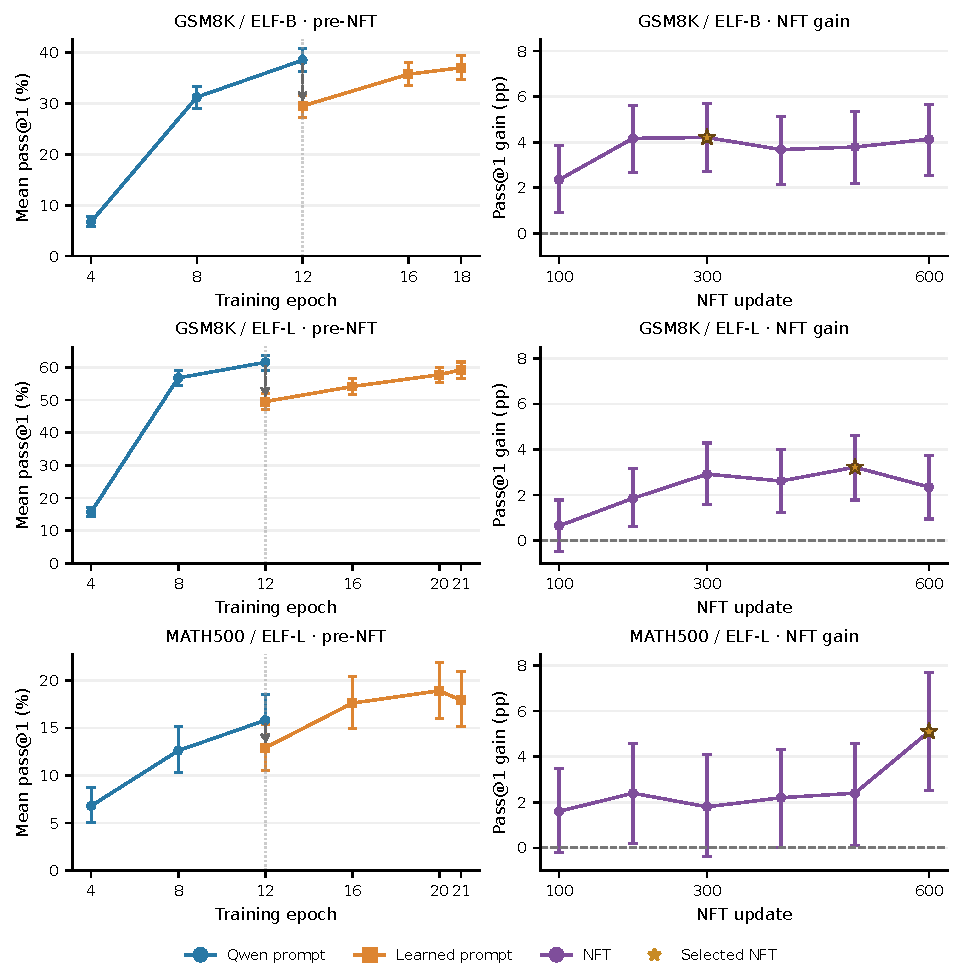
\includegraphics[width=.94\linewidth]{figures/training_curves_nft_improvement.pdf}
\caption{Supervised progress and subsequent NFT improvement. Left: absolute mean pass@1, with the epoch-12 prompt substitution shown explicitly. Right: paired gains over the final supervised checkpoint, with a common percentage-point axis and zero reference. Bars are pointwise 95\% problem-bootstrap intervals; stars mark development-selected NFT updates. Every point uses seeds 42/123 and 32 steps.}
\label{fig:trainingcurves}
\end{figure}

The supervised evaluations use ELF EMA $0.9999$, standalone prompt EMA $0.999$ at the immediate swap, and joint prompt EMA $0.9999$ thereafter. NFT evaluations use ELF/prompt EMA $0.99/0.99$. The reference for each NFT contrast is the final supervised checkpoint, not a separately evaluated NFT update-zero EMA state. Both ELF and the prompt encoder change during subsequent joint training, so these curves describe the complete training lineage rather than isolating prompt-encoder improvement. The two-seed curve values also differ from the four-seed prompt-stage comparison and eight-seed headline endpoints.

\section{Four-arm robustness to the inference clock}
\label{app:fourarm}
The main four-arm comparison uses shared $t=\tau^2$ inference for all arms. This reporting choice followed inspection of the test results and alignment with the shared-square control used in later-stage evaluations; it was not selected on an independent development set. Here we hold checkpoints, guidance, numerical arithmetic, and generation seeds fixed while changing the physical clock to $t=\tau$. Both schedules use 32 integration steps on the same base grid. The shared-square evaluator includes the $2\tau$ chain-rule factor; the identity evaluator uses the original scalar time embedding.

\begin{figure}[t]
\centering
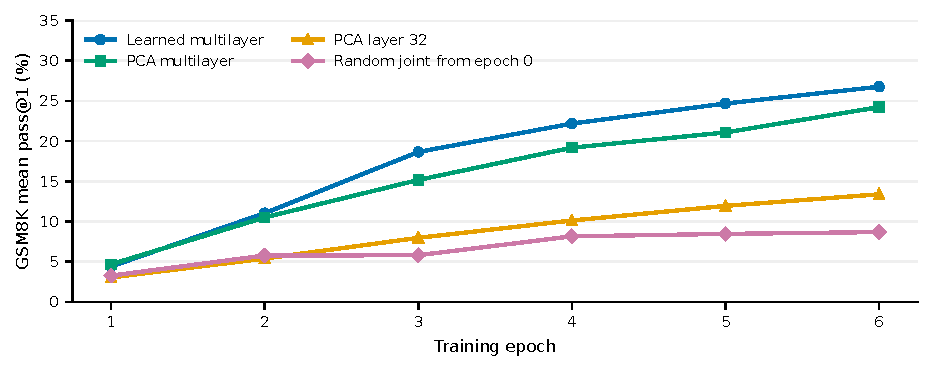
\includegraphics[width=\linewidth]{figures/four_arm_identity.pdf}
\caption{Identity-clock ($t=\tau$) counterparts of Figure~\ref{fig:fourarm}. Points average seeds 42/123 with the same trained checkpoints and EMA selectors. The epoch-six ordering is unchanged: learned multilayer, PCA multilayer, PCA layer 32, then random joint.}
\label{fig:fourarmidentity}
\end{figure}
% !TEX root = ../main.tex
\begin{table}[t]
\caption{Identity-clock ($t=\tau$) counterpart of the main four-arm comparison. Mean pass@1 (\%) over seeds 42/123, with 32 steps and ELF EMA $0.999$; random-joint prompt EMA is independently $0.999$. The epoch-six ordering agrees with shared $t=\tau^2$.}
\label{tab:identityfourarm}
\centering\small
\setlength{\tabcolsep}{4pt}
\begin{tabular}{rrrrr}
\toprule
Epoch & Learned multilayer & PCA multilayer & PCA layer 32 & Random joint \\
\midrule
1 & 4.40 & 4.66 & 3.03 & 3.26 \\
2 & 11.03 & 10.50 & 5.38 & 5.76 \\
3 & 18.65 & 15.16 & 7.96 & 5.80 \\
4 & 22.18 & 19.18 & 10.12 & 8.15 \\
5 & 24.68 & 21.08 & 11.94 & 8.45 \\
6 & 26.76 & 24.22 & 13.38 & 8.68 \\
\bottomrule
\end{tabular}
\end{table}

At epoch six, identity-clock accuracies are 26.76\%, 24.22\%, 13.38\%, and 8.68\% for learned multilayer, PCA multilayer, PCA layer 32, and random joint, respectively. Learned multilayer exceeds PCA multilayer from epoch two onward under both schedules; multilayer PCA exceeds layer 32 PCA at every epoch. Shared $t^2$ improves the two multilayer teacher-prompt arms at later checkpoints but does not uniformly help: layer 32 PCA decreases at epochs four through six, and random joint remains weak. We therefore interpret the persistent endpoint ordering as robustness of these ablation conclusions to the two tested clocks, rather than a general advantage of a squared clock.

All arms use the original seed-42 ELF initialization, 2,434,330 training rows, effective batch 512, and fresh optimizers. The PCA multilayer run migrated from two to four GPUs during training while preserving effective batch; this changed its stochastic trajectory. No arm is repeated to estimate training variability. The representation comparisons hold layer selection fixed for learned versus PCA projectors and projector family fixed for multilayer versus layer 32; they do not measure the interaction between the two choices.

% !TEX root = ../main.tex
\begin{table}[t]
\caption{Identity-clock epoch-six representation results with four seeds (42/123/456/789), matching the seed set of the primary shared-$t^2$ table. All rows use original Qwen conditioning, ELF EMA $0.999$, and 32 steps.}
\label{tab:identityfourseed}
\centering\small
\setlength{\tabcolsep}{4pt}
\begin{tabular}{lrrr}
\toprule
Representation & Pass@1 (\%) & Pass@2 (\%) & Pass@4 (\%) \\
\midrule
Learned multilayer & 27.05 & 38.22 & 49.43 \\
PCA multilayer & 23.98 & 35.06 & 46.25 \\
PCA layer 32 & 13.04 & 20.33 & 29.64 \\
\bottomrule
\end{tabular}
\end{table}

A separate identity-clock epoch-six extension evaluates the three teacher-prompt representation arms with four generation seeds (Table~\ref{tab:identityfourseed}). Learned minus PCA multilayer is $+3.07$ points with paired 95\% interval $[1.57,4.51]$; PCA multilayer minus layer 32 is $+10.94$ points, $[9.44,12.51]$. These intervals condition on the trained checkpoints and observed draws. Both four-seed clock comparisons support the representation ordering; each uses its own predictions and bootstrap contrasts.

% !TEX root = ../main.tex
\begin{table}[t]
\caption{Four-seed shared-$t^2$ epoch-six results extending Table~\ref{tab:representation}. All entries are percentages. Pass@2 and pass@4 measure oracle coverage over the same four draws; bracketed ranges are 95\% problem-bootstrap intervals.}
\label{tab:shared2multisample}
\centering\small
\setlength{\tabcolsep}{4pt}
\begin{tabular}{lrrr}
\toprule
Arm & Pass@1 & Pass@2 [95\% CI] & Pass@4 [95\% CI] \\
\midrule
Learned multilayer & 30.76 & 42.03 [39.68, 44.24] & 53.22 [50.57, 55.88] \\
PCA multilayer & 28.43 & 39.13 [36.85, 41.32] & 50.11 [47.46, 52.77] \\
PCA layer 32 & 11.20 & 17.15 [15.43, 18.84] & 24.18 [21.91, 26.38] \\
Random joint & 8.70 & 13.61 [12.03, 15.21] & 20.02 [17.82, 22.21] \\
\bottomrule
\end{tabular}
\end{table}

% !TEX root = ../main.tex
\begin{table}[t]
\caption{Individual sampling-seed accuracies (\%) for the shared-$t^2$ epoch-six comparison. These are generation seeds at fixed trained checkpoints, not independent training runs.}
\label{tab:shared2seeds}
\centering\small
\setlength{\tabcolsep}{4pt}
\begin{tabular}{lrrrr}
\toprule
Arm & Seed 42 & Seed 123 & Seed 456 & Seed 789 \\
\midrule
Learned multilayer & 30.71 & 31.31 & 30.63 & 30.40 \\
PCA multilayer & 28.58 & 28.20 & 28.58 & 28.35 \\
PCA layer 32 & 11.52 & 11.83 & 10.69 & 10.77 \\
Random joint & 8.57 & 8.64 & 8.42 & 9.17 \\
\bottomrule
\end{tabular}
\end{table}

Tables~\ref{tab:shared2multisample} and~\ref{tab:shared2seeds} give oracle coverage and individual seed accuracies for the primary shared-$t^2$ epoch-six comparison. All four arms use the same four generation seeds. Learned minus PCA multilayer is $+2.89$ points at pass@2 (paired 95\% interval $[1.10,4.76]$) and $+3.11$ at pass@4 ($[0.68,5.54]$). The four-arm ordering also persists in these oracle-coverage metrics. These additional draws improve evaluation precision without measuring variability across training runs.

\section{Broader inference-schedule sweep}
\label{app:schedules}
% !TEX root = ../main.tex
\begin{table}[t]
\caption{Broader ELF-L schedule sweep at 32 steps, seeds 42/123. This two-seed table is separate from the four-seed primary schedule comparison. Entries are mean pass@1 (\%). The two epoch-21 columns use supervised states; NFT columns use the selected post-training endpoints.}
\label{tab:schedulestwoseed}
\centering\small
\begin{tabular}{lrrrr}
\toprule
Layer clocks & GSM8K e21 & GSM8K NFT & MATH e21 & MATH NFT \\
\midrule
$(1.0,1.0,1.0)$ & 52.96 & 58.72 & 15.50 & 20.90 \\
$(1.5,1.5,1.5)$ & 57.35 & 62.32 & 18.10 & 23.50 \\
$(2.0,2.0,2.0)$ & 57.51 & 62.81 & 17.40 & 20.40 \\
$(2.5,2.5,2.5)$ & 55.80 & 61.41 & 18.10 & 20.20 \\
$(2.5,2.0,1.5)$ & 59.25 & 62.47 & 17.90 & 23.00 \\
$(1.5,2.0,2.5)$ & 58.07 & 62.85 & 17.60 & 22.20 \\
\bottomrule
\end{tabular}
\end{table}

Table~\ref{tab:schedulestwoseed} retains all six schedules evaluated with seeds 42/123. Table~\ref{tab:schedules} in the main paper extends the headline async allocation and the two competitive shared exponents, 1.5 and 2, to four seeds. The two tables summarize different draw sets. In particular, the two-seed MATH NFT async-minus-shared-$t^2$ difference of $+2.60$ points becomes $+0.65$ points with four seeds, with interval $[-0.60,1.85]$. Neither sweep establishes a universally optimal schedule. These are inference-clock comparisons at fixed trained checkpoints, separate from the NFT rollout-clock experiments below.

\section{SCCFG sensitivity at the supervised endpoint}
\label{app:sccfgsweep}
We sweep SCCFG coefficients $\{1,2,3,4\}$ at the epoch-21 ELF-L checkpoints on GSM8K and MATH500. Both use ELF/prompt EMA $0.9999/0.9999$, async $(2.5,2,1.5)$, 32 steps, CFG 1, and seeds 42/123. The coefficient is applied to both denoising and terminal decoding; SCCFG 1 retains recurrent self-conditioning. Separate seeded invocations match the initial noise across coefficients.

\begin{figure}[t]
\centering
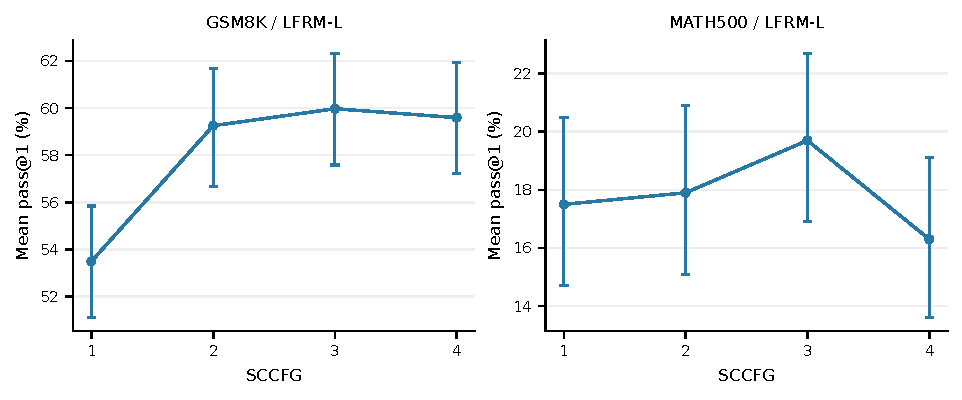
\includegraphics[width=\linewidth]{figures/sccfg_sweep.pdf}
\caption{SCCFG sensitivity on full GSM8K and MATH500 test sets at ELF-L epoch 21. Points average seeds 42/123; bars show pointwise 95\% problem-bootstrap intervals for absolute pass@1. Other inference settings and checkpoints are fixed. This is a test-set sensitivity analysis; the headline setting remains SCCFG 2.}
\label{fig:sccfgsweep}
\end{figure}

SCCFG 3 gives the highest observed mean on both tasks: 59.97\% on GSM8K and 19.70\% on MATH500, compared with 59.25\% and 17.90\% at SCCFG 2. The paired improvements over 2 are $+0.72$ points ($[-0.49,1.93]$) and $+1.80$ ($[-0.20,3.80]$), respectively; both intervals include zero. On GSM8K, reducing SCCFG from 2 to 1 lowers accuracy by 5.76 points ($[4.36,7.13]$). This sweep characterizes sensitivity at these checkpoints without establishing a universally optimal coefficient.

\section{Prompt-stage results and imitation curves}
\label{app:prompt}
\begin{table}[t]
\caption{Four-seed prompt-stage comparison at 32 steps. ELF EMA is $0.9999$; the swapped MSE prompt uses $0.999$, and the joint prompt uses $0.9999$.}
\label{tab:promptstage}
\centering\small
\begin{tabular}{lrrr}
\toprule
Benchmark / model & Qwen epoch 12 & MSE swap & Joint endpoint \\
\midrule
GSM8K / ELF-B & 38.25 & 29.34 & 37.77 \\
GSM8K / ELF-L & 60.78 & 49.07 & 58.53 \\
MATH500 / ELF-L & 16.00 & 13.20 & 17.45 \\
\bottomrule
\end{tabular}
\end{table}

The immediate swap losses are $8.91$ points for GSM8K ELF-B (95\% paired interval $[7.32,10.52]$), $11.71$ for GSM8K ELF-L ($[10.08,13.42]$), and $2.80$ for MATH ($[1.10,4.45]$). Subsequent joint gains are $8.43$ ($[6.96,10.01]$), $9.46$ ($[7.83,11.05]$), and $4.25$ ($[2.50,6.05]$). Final joint minus original-Qwen accuracy is $-0.47$, $-2.26$, and $+1.45$ points, respectively. Their paired intervals are $[-2.09,1.18]$, $[-3.90,-0.64]$, and $[-0.25,3.30]$.

\begin{figure}[t]
\centering
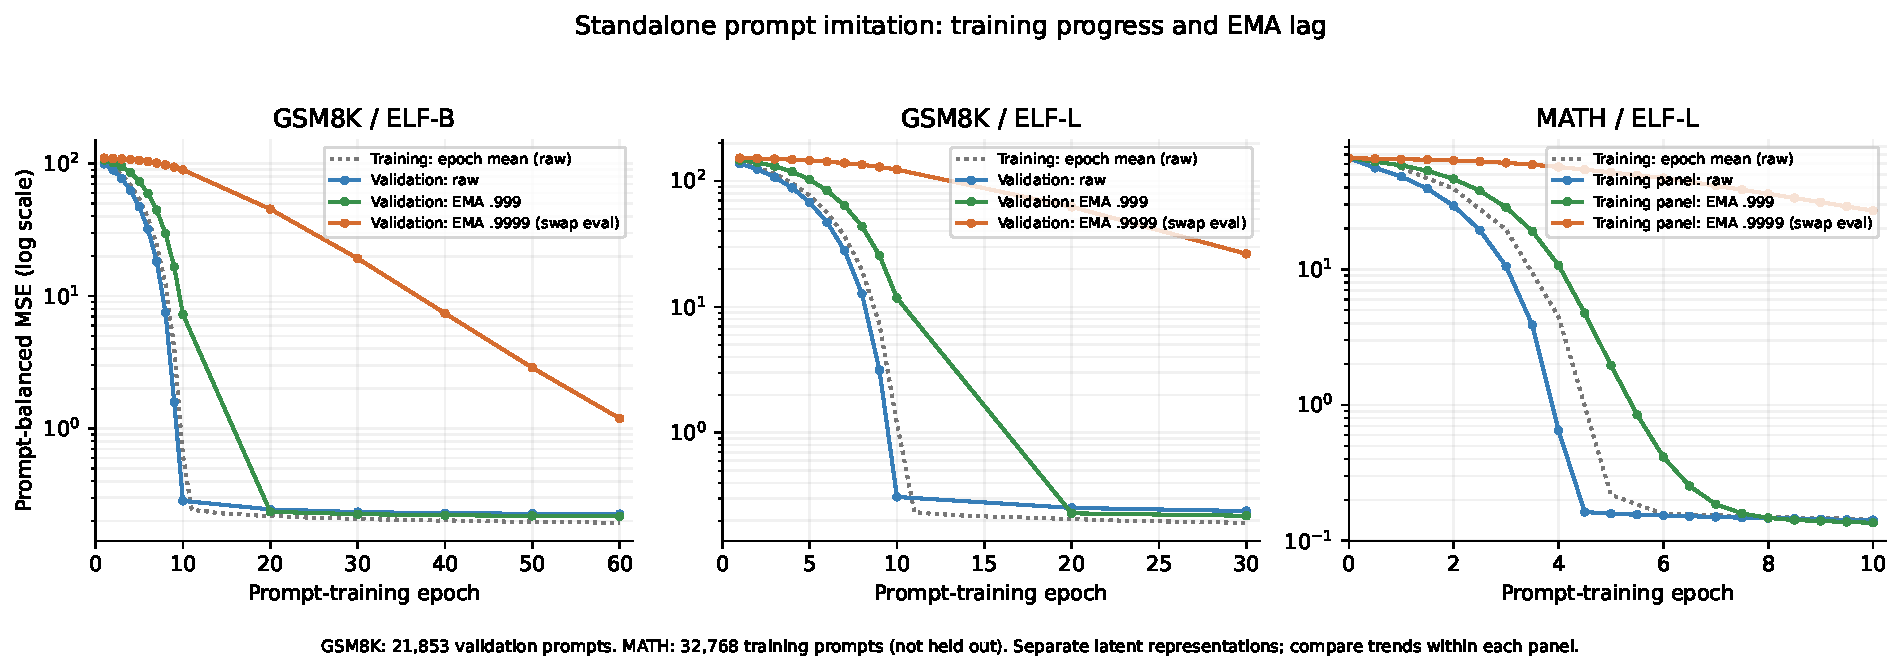
\includegraphics[width=\linewidth]{figures/prompt_mse.pdf}
\caption{Standalone prompt-imitation progress. GSM8K curves use 21,853 held-out prompts; MATH evaluation uses a fixed 32,768-prompt training diagnostic panel. Prompt-training epochs differ from denoiser epochs. Each task has its own target representation, so absolute losses should not be compared across panels.}
\label{fig:promptmse}
\end{figure}
The final prompt EMA $0.999$ MSEs are 0.2172, 0.2191, and 0.1356 for the three models. The corresponding $0.9999$ losses are 1.1899, 26.3952, and 27.0031. The slower EMA therefore remains a poor proxy for the fitted prompt at these endpoints. Figure~\ref{fig:promptmse} shows why the primary swap comparison uses $0.999$. The curves document training progress and diminishing improvements where observed; they do not establish convergence of every EMA track.

\section{Layer-choice motivation and robustness}
\label{app:cka}
\begin{figure}[t]
\centering
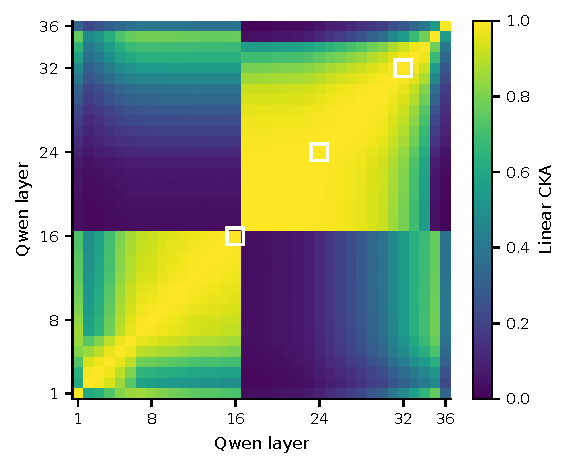
\includegraphics[width=.62\linewidth]{figures/cka.pdf}
\caption{Linear CKA across the frozen teacher's 36 post-block representations. White diagonal markers identify layers 16, 24, and 32. The pronounced transition after layer 16 motivates including it; layers 24 and 32 sample progressively deeper representations at regular intervals.}
\label{fig:cka}
\end{figure}
The CKA study uses two disjoint 4,096-problem panels of teacher-forced gold solutions. Assistant-content activations are mean-pooled into eight relative-position bins, concatenated, and compared with equal weight per problem. The selected layers have pairwise CKA 0.124 (16/24), 0.543 (16/32), and 0.842 (24/32), while the adjacent 16/17 value is 0.038. CKA motivates a practical choice across depth; it is not an optimization criterion for downstream accuracy.

We also probe the frozen teacher by perturbing assistant activations at one selected layer at a time, with noise magnitude proportional to each problem's clean activation RMS. The 64-problem GSM8K panel is stratified by token length and uses two noise seeds. Gold-token CE, teacher-distribution KL, and top-1 agreement measure downstream deterioration. This diagnostic combines sensitivity at the intervened layer with recovery through the remaining teacher suffix. It therefore does not directly predict the best clocks for the trained ELF denoiser, whose projected coordinates and conditional dynamics differ from those of Qwen.

\section{Sampling cost and pre-NFT tradeoffs}
\label{app:cost}
\begin{figure}[t]
\centering
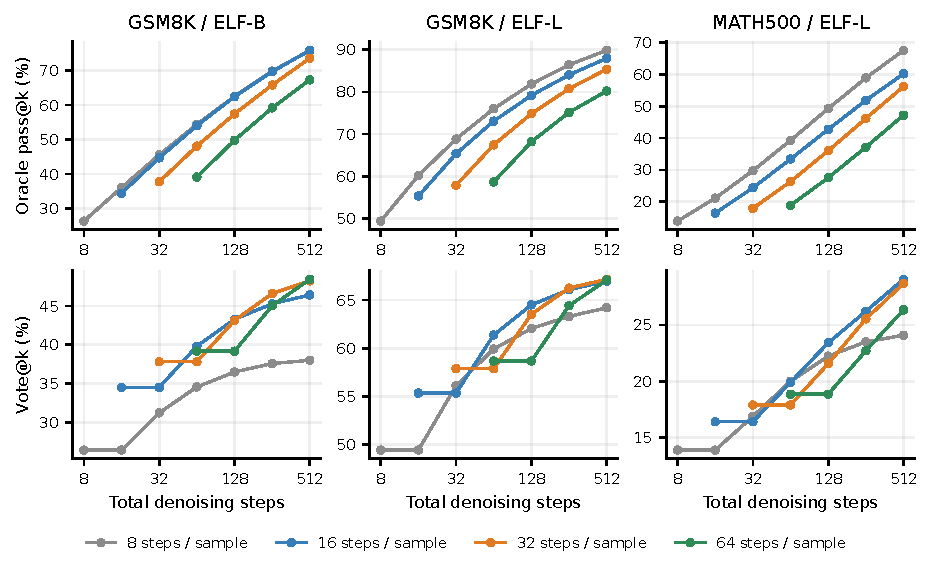
\includegraphics[width=\linewidth]{figures/pre_budget.pdf}
\caption{Supervised endpoint counterparts of Figure~\ref{fig:budget}, with the same sample budgets and asynchronous clocks. Upper panels show oracle coverage and lower panels show final-answer voting.}
\label{fig:prebudget}
\end{figure}
\begin{figure}[t]
\centering
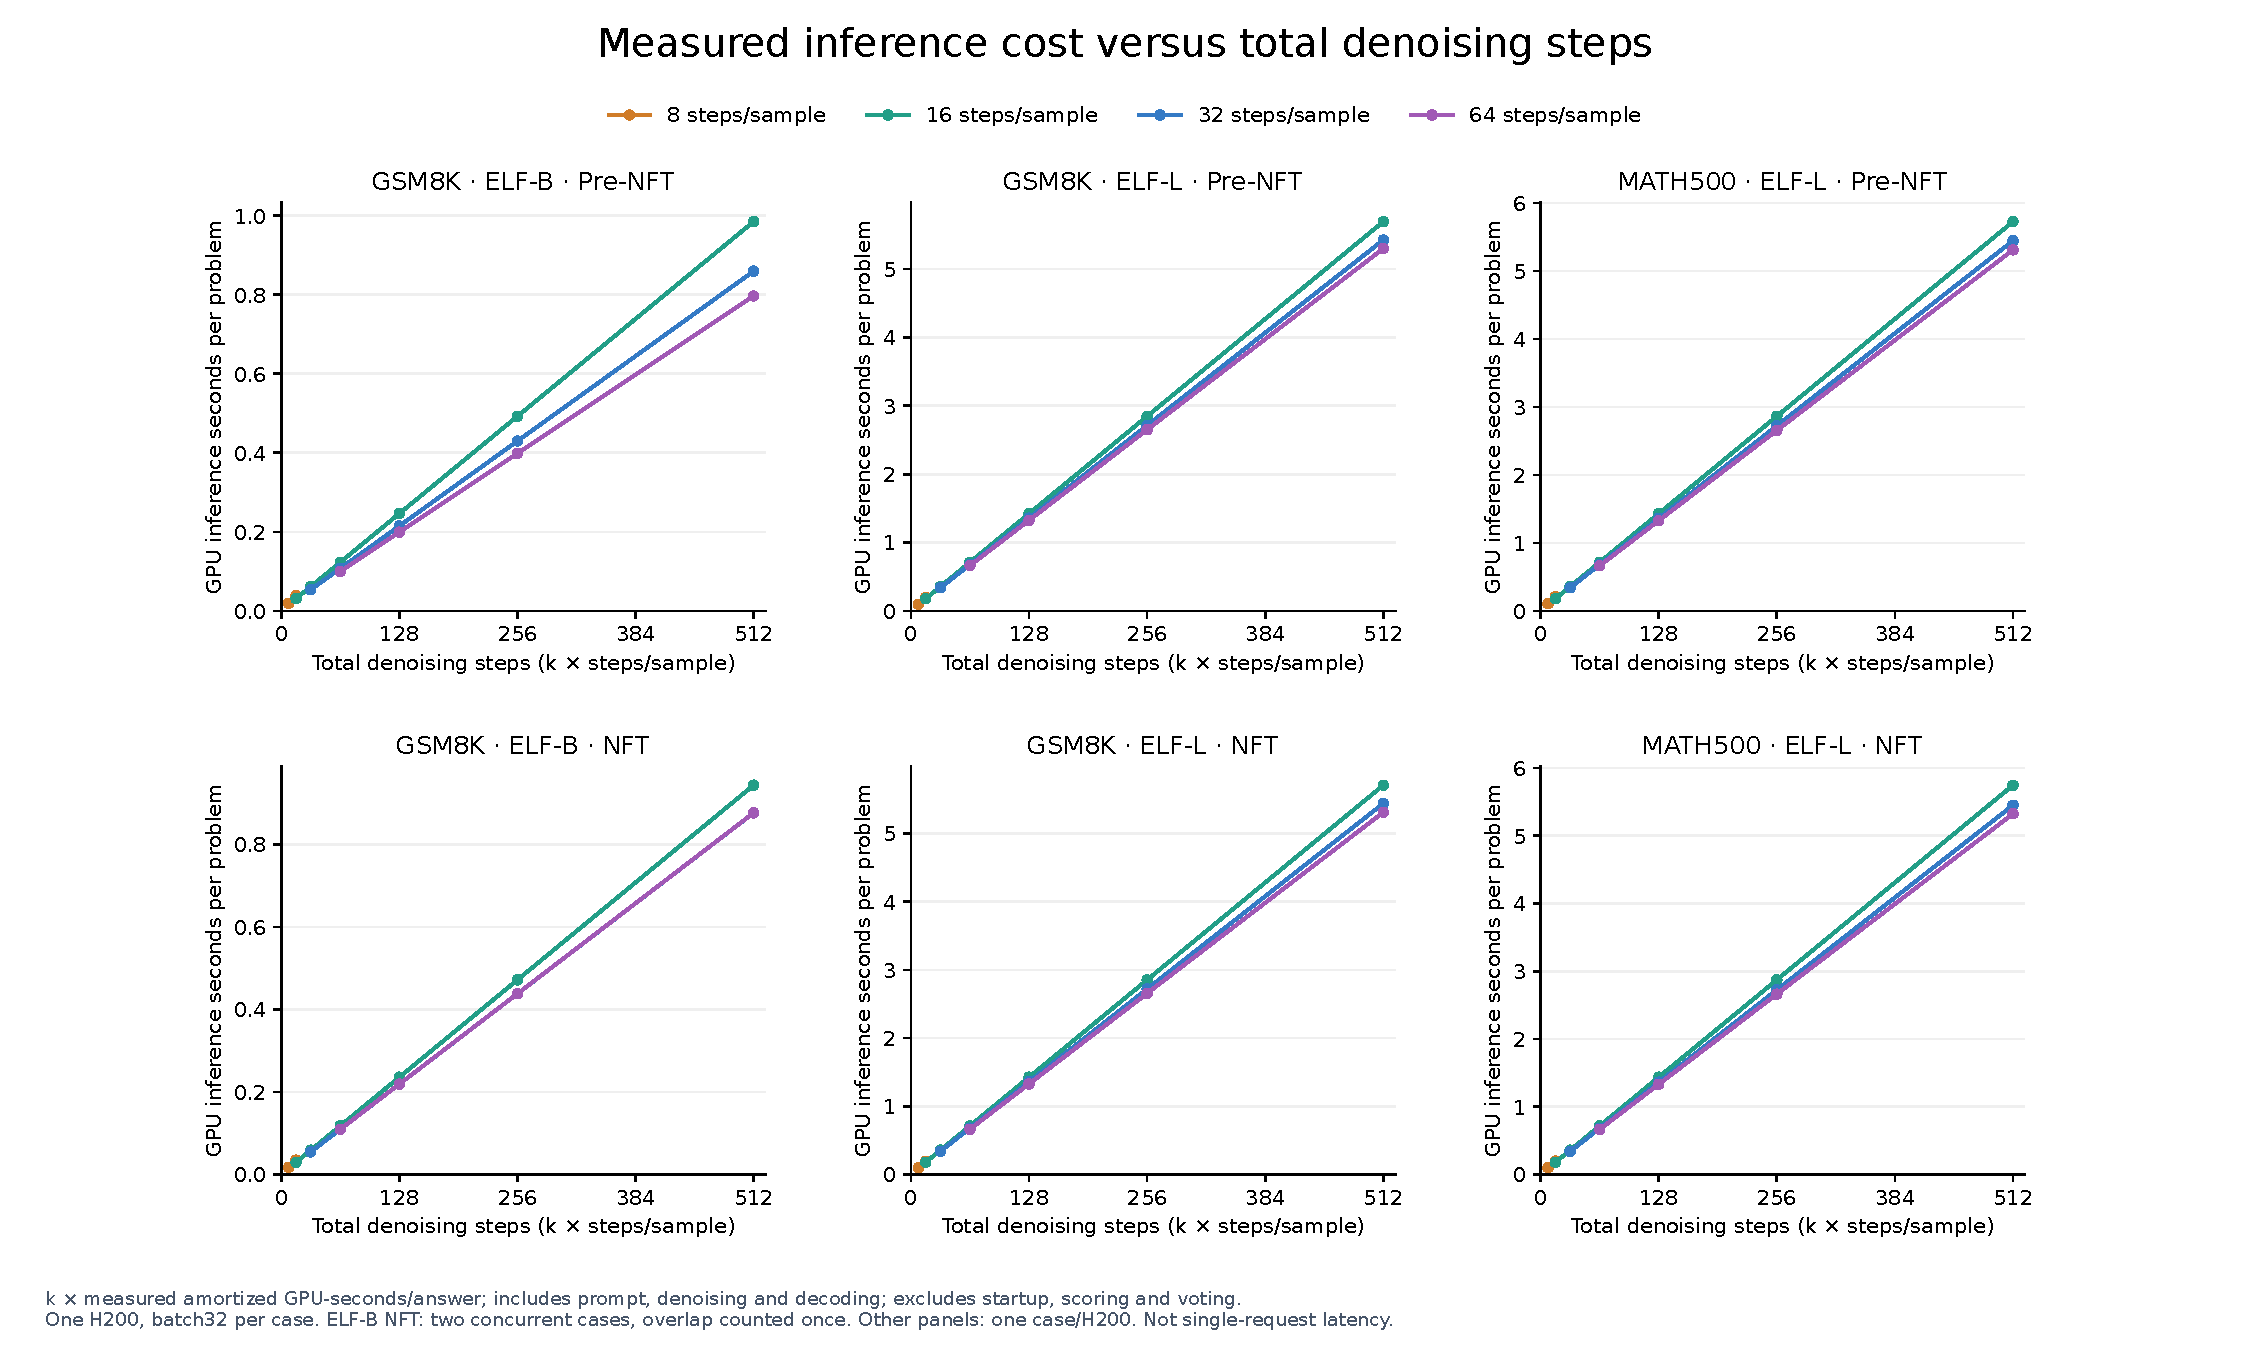
\includegraphics[width=\linewidth]{figures/time_vs_steps.pdf}
\caption{Measured GPU inference time against total denoising steps, including the expanded 8-step cohorts with 64 draws. All four depths reach 512 total steps at all six endpoints. Time includes prompt encoding, denoising, and terminal decoding, while excluding startup, scoring, and voting. These are throughput-derived amortized costs, not single-query latencies. ELF-B NFT runs pack two cases on one H200; the other panels use one case per H200.}
\label{fig:time}
\end{figure}
The timing analysis uses 23,832 recorded batch inference windows from 716 of the 720 seed evaluations. Four older GSM NFT seed cases have no recorded timing; later compatible draws supply the corresponding timing coefficients. Missing measurements are not imputed as zero. Within each cohort, we union overlapping inference windows per GPU allocation and divide their summed durations by the total measured answer count. Multiplying this amortized cost by the number of draws gives each plotted point. This avoids double-counting concurrent ELF-B NFT workers. At a fixed denoising-step budget, shorter trajectories require more prompt-encoder and terminal-decoder work because they generate more samples. This explains the systematic overhead visible in Figure~\ref{fig:time} and motivates reporting both steps and measured cost.

\section{Answer diversity, coverage, and NFT filtering}
\label{app:diversity}
\begin{figure}[t]
\centering
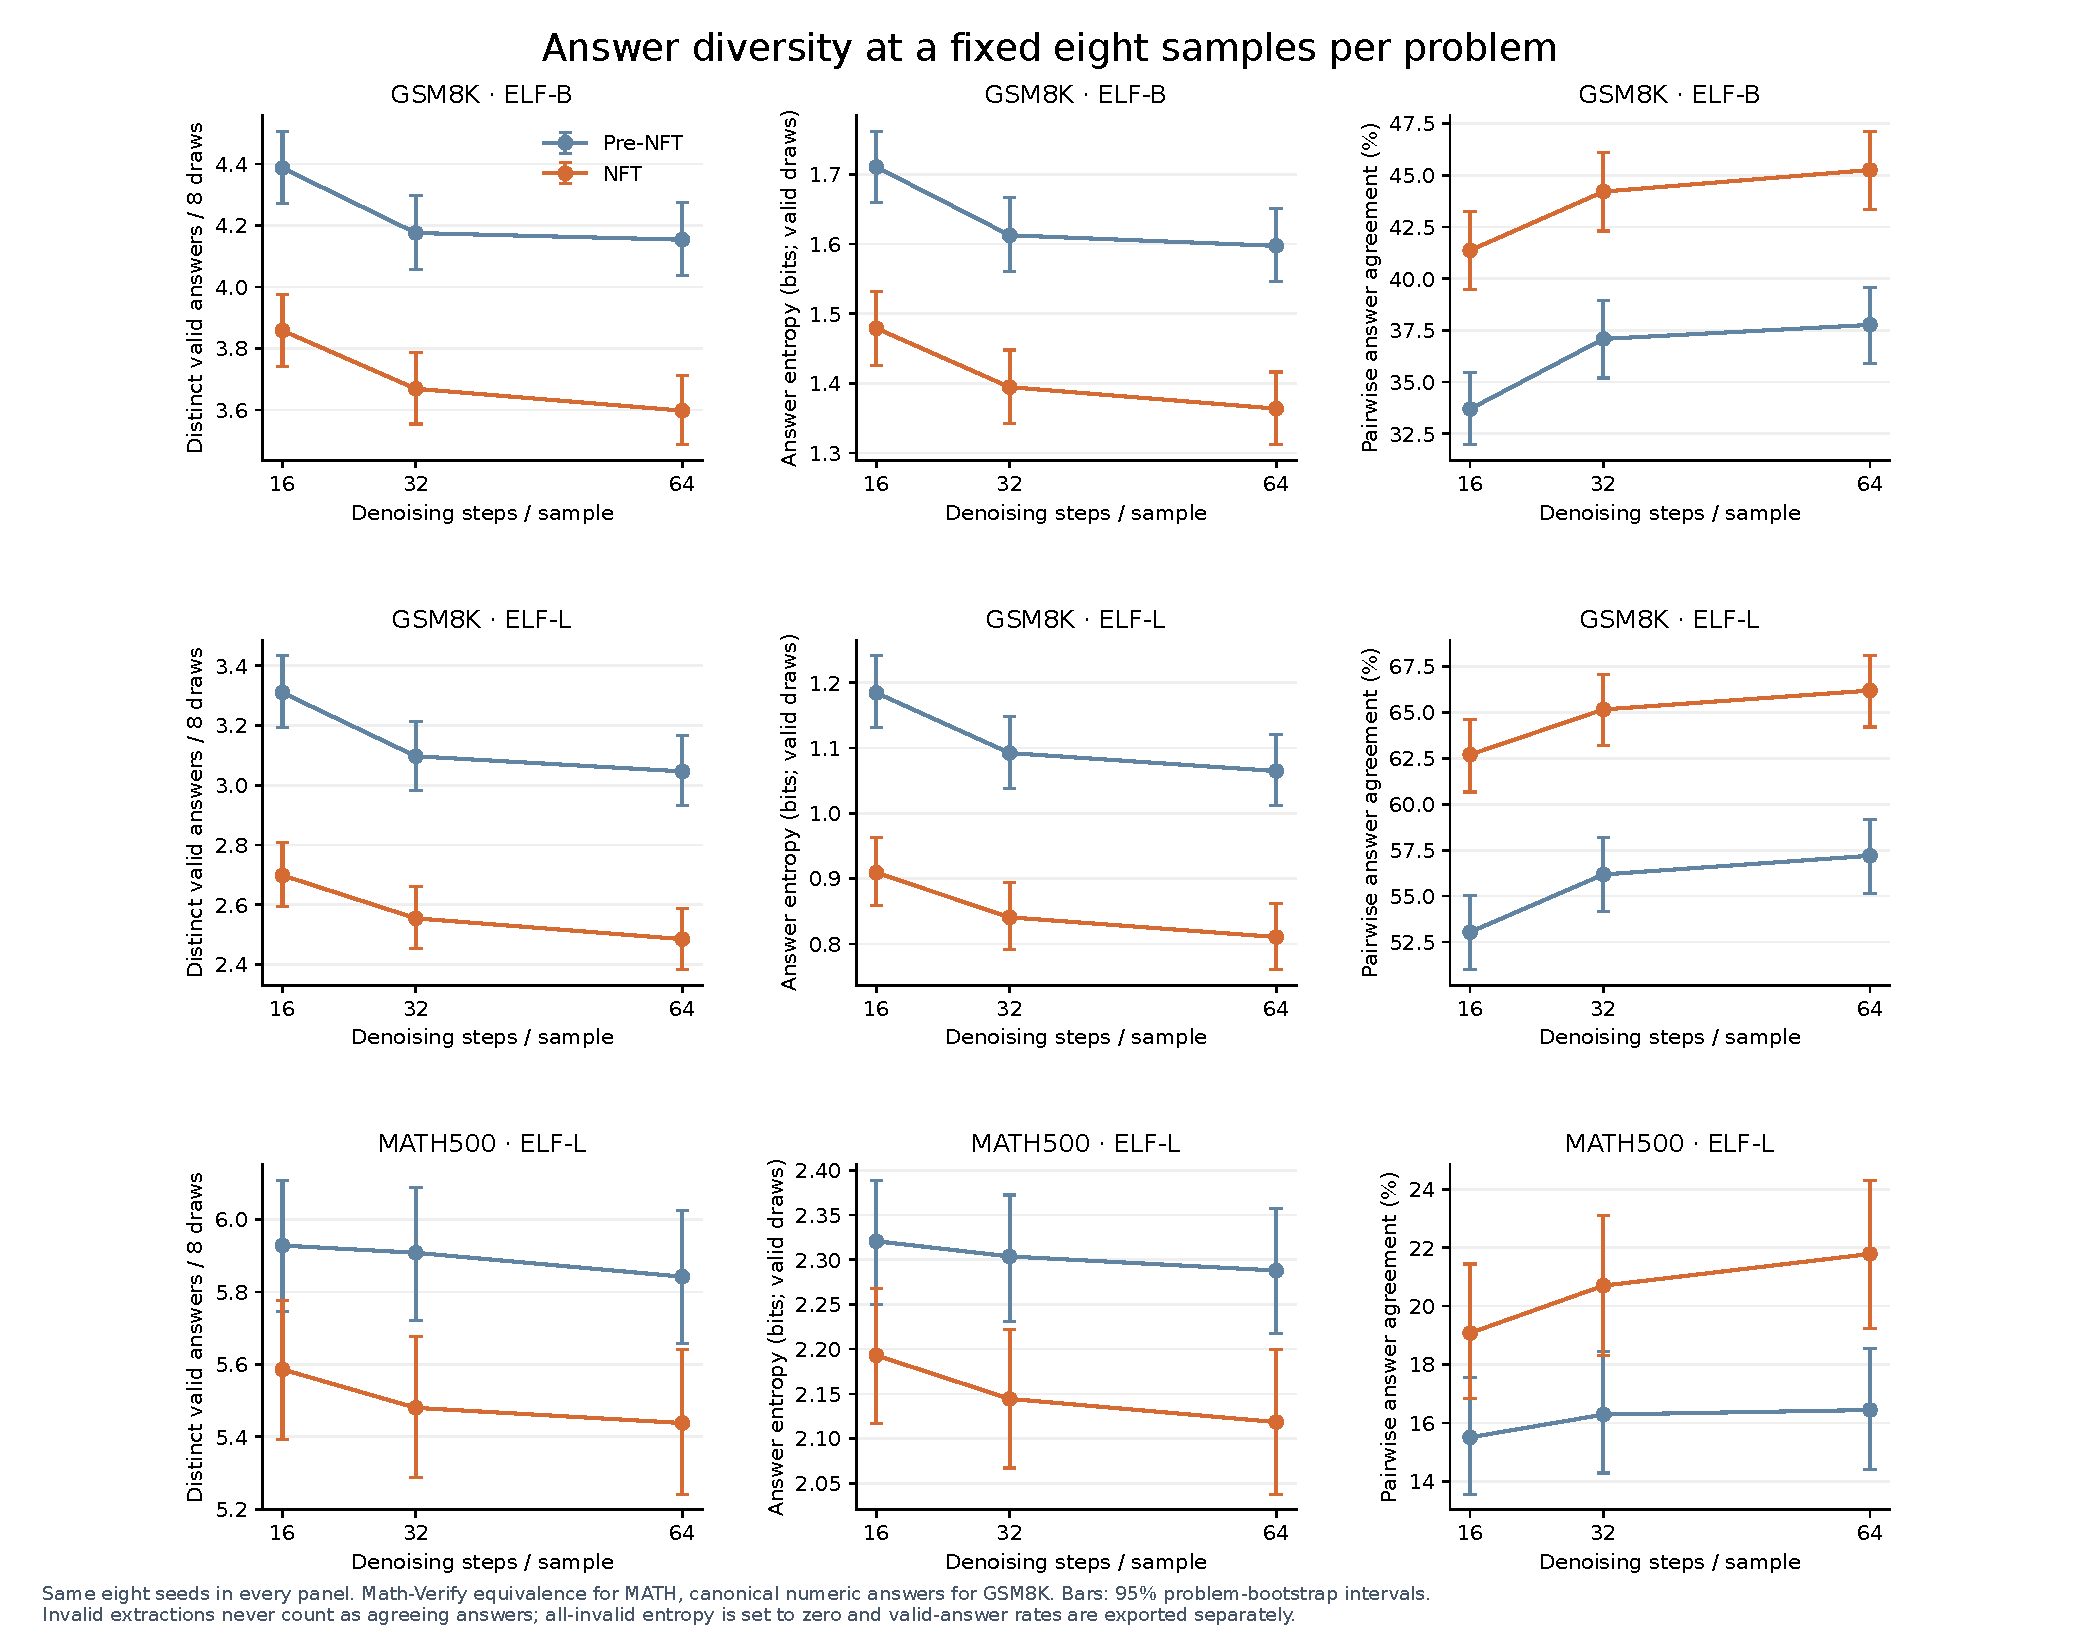
\includegraphics[width=\linewidth]{figures/diversity.pdf}
\caption{Answer diversity before and after NFT. The fixed-eight-sample comparison holds the number of draws constant. Diversity concerns extracted final answers, not the semantic diversity of reasoning paths.}
\label{fig:diversity}
\end{figure}
\begin{figure}[t]
\centering
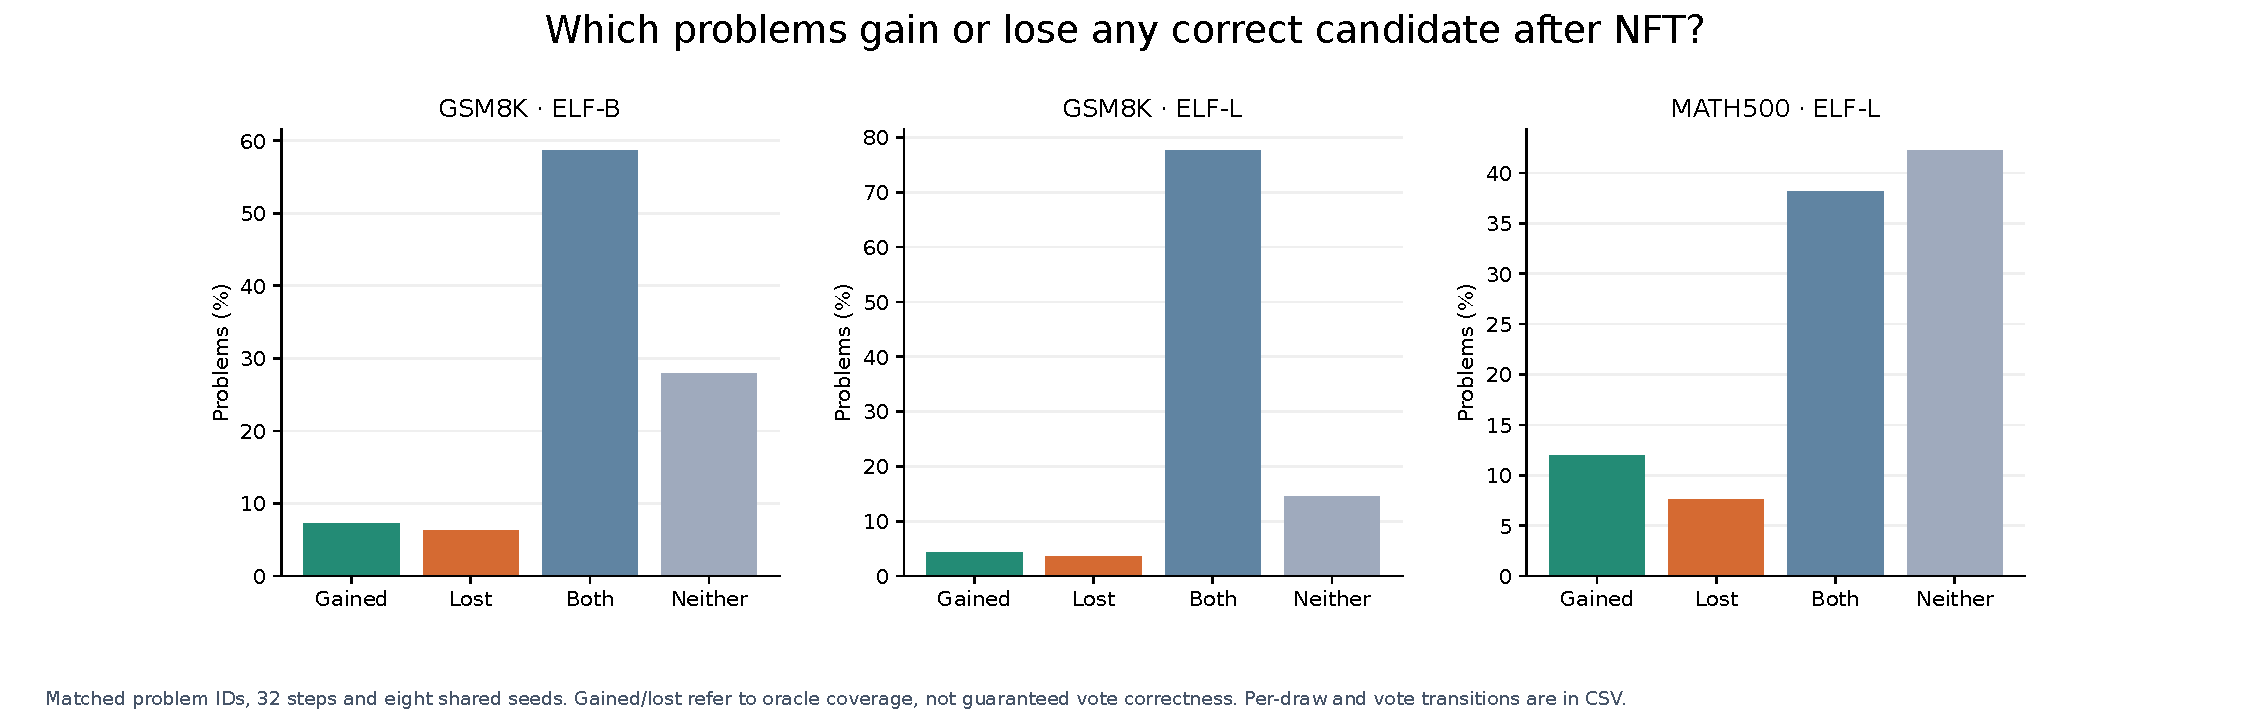
\includegraphics[width=\linewidth]{figures/coverage_transitions.pdf}
\caption{Problem-level coverage transitions between supervised and NFT endpoints, using matched generation cohorts. Aggregate improvements can coexist with problems that lose coverage.}
\label{fig:transitions}
\end{figure}
\begin{figure}[t]
\centering
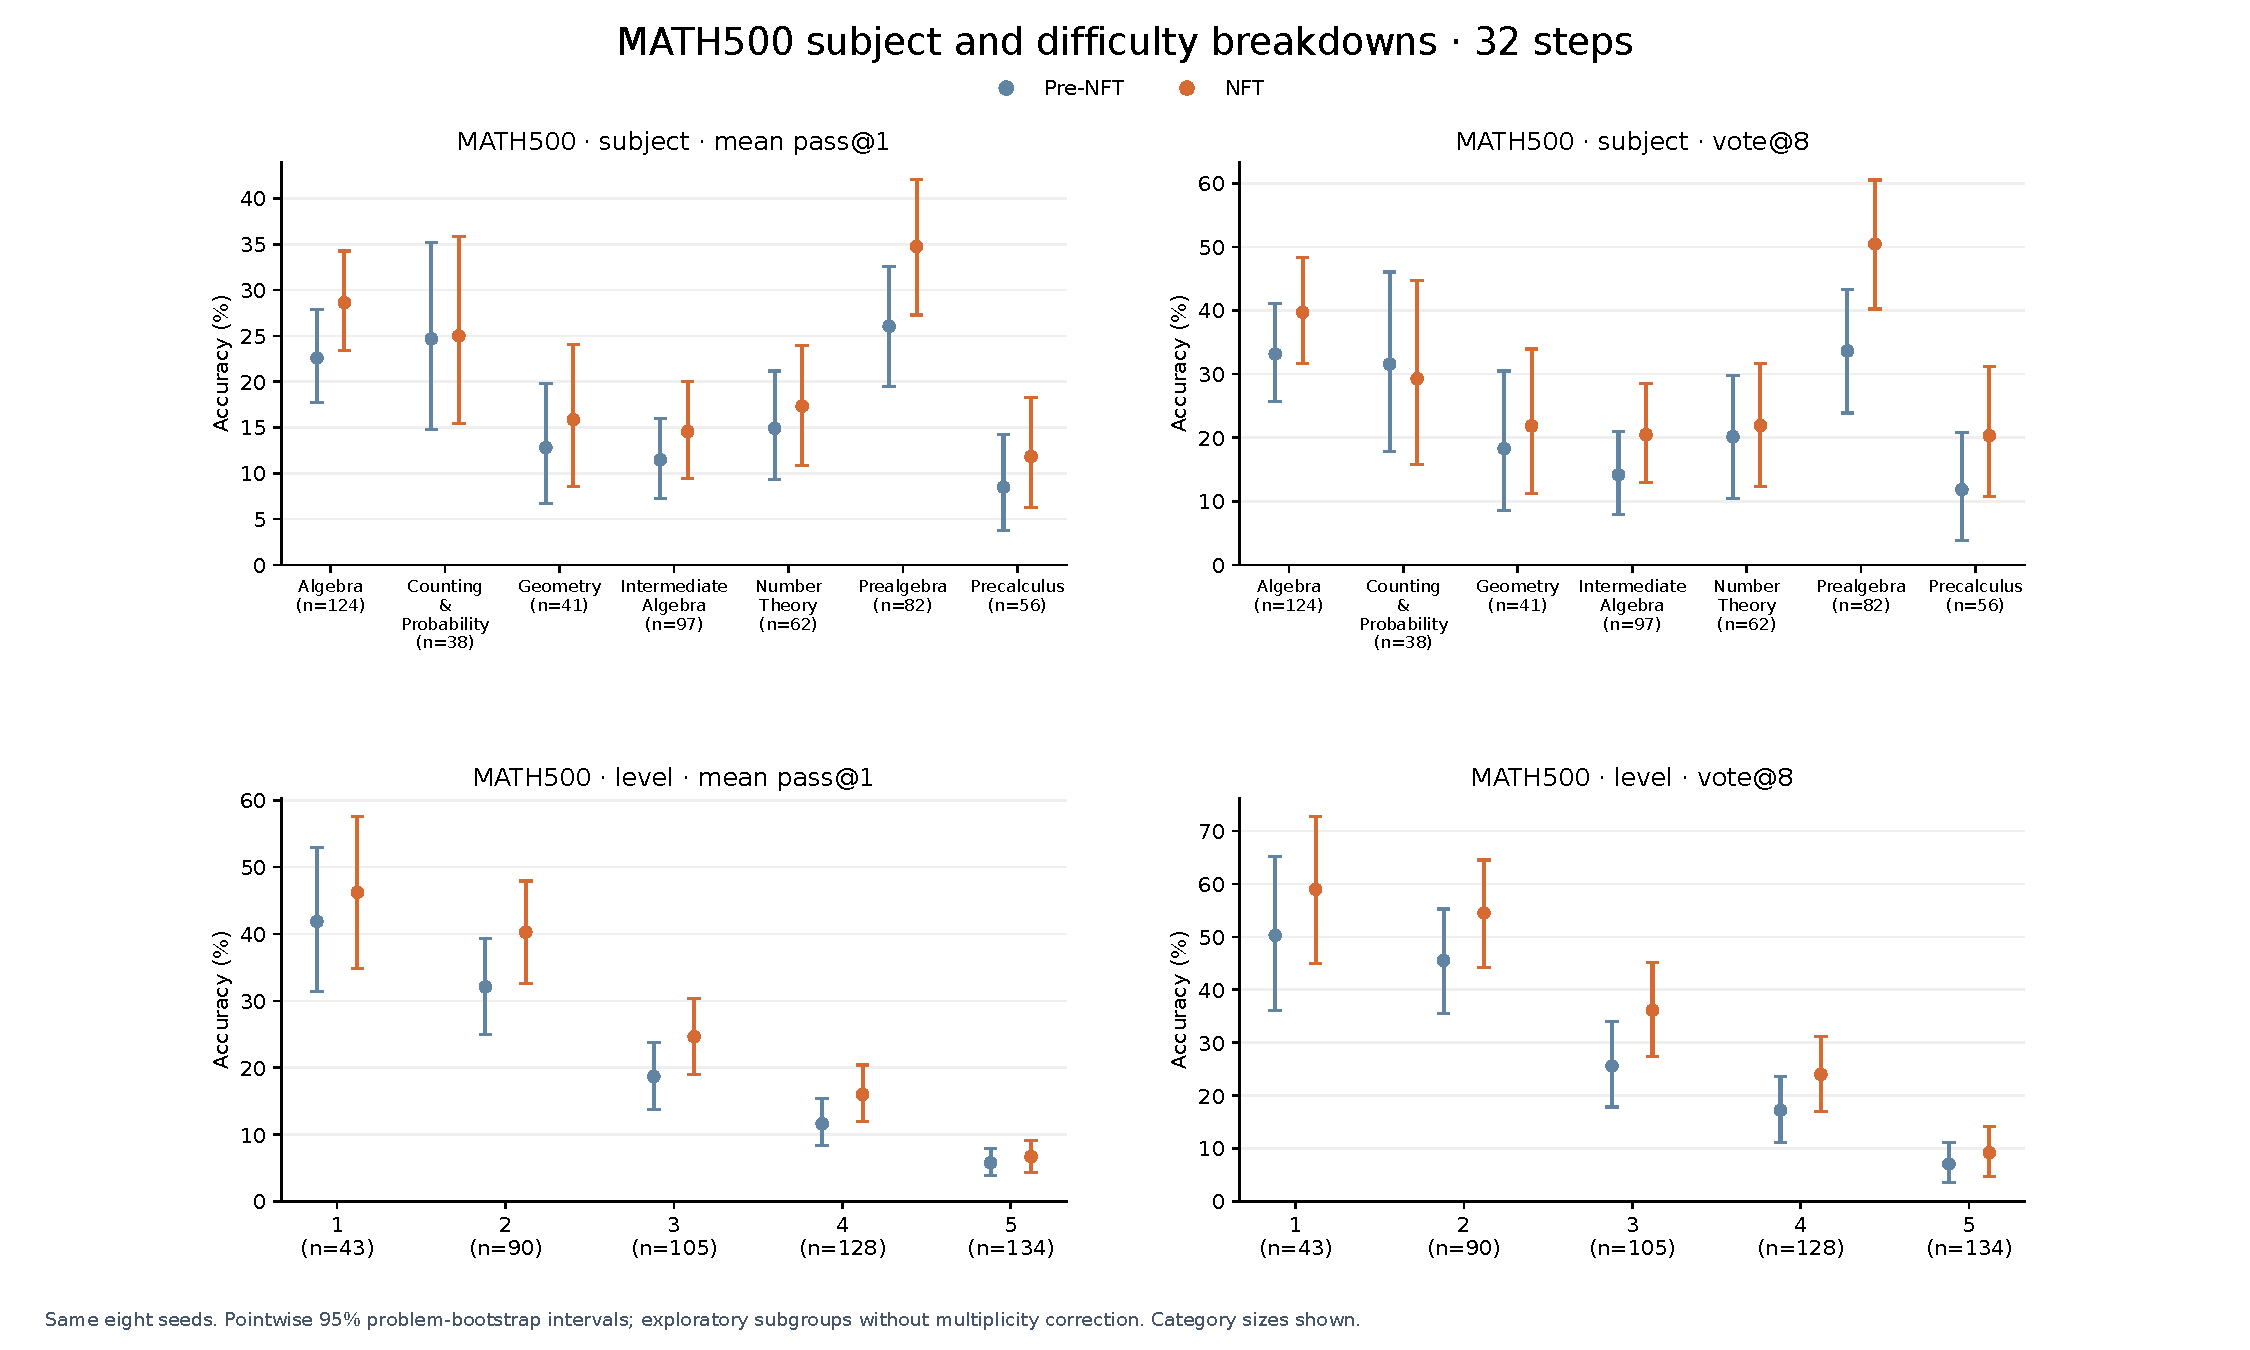
\includegraphics[width=\linewidth]{figures/math_breakdown.pdf}
\caption{Exploratory MATH500 subject and difficulty breakdowns from the saved predictions. Subgroups are smaller than the full benchmark and are descriptive analyses, not separately selected evaluation endpoints.}
\label{fig:mathbreakdown}
\end{figure}

For the first 200 NFT updates, discarded all-correct groups comprise 20.10\% for GSM8K ELF-B, 38.81\% for GSM8K ELF-L, and 1.44\% for MATH ELF-L. Through the selected endpoints, these fractions are 22.32\%, 43.50\%, and 1.81\%, respectively. Each retained group supplies the same number of endpoint/time records, so a lower discard fraction leaves more training records per update. The token mass can still differ because answers have different lengths. The smaller discard rate on MATH is consistent with broader training coverage contributing to its NFT gains, but this comparison does not isolate a causal filtering effect.

An additional GSM8K ELF-B rollout comparison uses shared-square $(2,2,2)$ versus identity $(1,1,1)$ clocks during NFT collection, with synchronous loss times in both arms. Through update 400, shared-square discards 31.84\% of groups versus 23.55\% for identity; matched asynchronous test accuracy is 39.12\% versus 40.75\%. Identity is also ahead at update 200, while shared-square is ahead at update 100 with one evaluation seed. This supports recording rollout difficulty and discarded fraction together, without attributing the accuracy difference solely to filtering.

\clearpage
% !TEX root = ../main.tex
\section{Literature comparisons and evaluation protocols}
\label{app:literature}
We organize the literature available through September 19, 2026 by generative representation, inference structure, and evaluation protocol. The tables below reproduce selected operating points from primary papers; they are not evaluations performed with our harness. A model name alone is insufficient to identify a result: checkpoint, prompting, output length, sampling order, and post-training can all change the reported score. In particular, a paper's \emph{MATH} result is not automatically a MATH500 result. We retain the distinction even when later papers place the numbers in a shared column.

\subsection{Continuous models and small-model comparisons}
\label{app:literaturecontinuous}
The continuous-flow rows in Table~\ref{tab:literature} have different operating points. $\mathbb S$-FLM uses top-1 velocity, temperature one, and 1,024 sampling steps (its Table~2). FMLM+ initialized from an MDLM reaches 33.6\% at 64 function evaluations; its scratch and distillation variants reach 19.1\% and 23.4\%, respectively (its Table~8). Both papers train on TinyGSM and execute generated Python solutions \citep{hyperspherical,posterior}. MLFM adapts a frozen 1,028M-parameter SMDM backbone with additional adapters; its 31.24\% result uses continuous classifier-free guidance, online token promotion, and 256 sampling steps, with a 512-token limit \citep{mlfm}. It retains discrete token promotion within a continuous trajectory, whereas our model decodes the complete answer at the end.

Early work also establishes mathematical reasoning in diffusion models. Diffusion of Thoughts reports 32.6\% for Plaid and 53.5\% for SEDD-medium on its GSM8K-Aug protocol, with separate self-consistency scores \citep{dot}. DiffuGPT-M reports 61.8\% with 355M parameters under a symbolic-reasoning protocol \citep{diffugpt}. These results are relevant precedents, but their compact reasoning format differs from our natural-language solution format. SMDM's 58.5\% likewise follows task-specific augmented-GSM8K fine-tuning \citep{smdm}. Duo's 1.7B result follows large-scale pretraining and supervised mathematical adaptation \citep{duoscaling}.

\begin{table}[ht]
\caption{Additional small diffusion models. Scores are percentages. ``MATH'' retains the original paper's label and is deliberately separate from MATH500. Rows marked $^*$ are the evaluations reported in OPDLM's Table~6, rather than the original model paper.}
\label{tab:literaturesmall}
\centering\small
\begin{tabular}{lrrrr}
\toprule
Model & Params (B) & GSM8K & MATH500 & MATH\\
\midrule
Simple-dLLM, masked \citep{simpledllm} & 0.6 & 29.30 & --- & 8.70\\
Simple-dLLM, block \citep{simpledllm} & 0.6 & 46.30 & --- & 12.90\\
Simple-dLLM, block$^*$ \citep{opdlm} & 0.6 & 46.30 & 15.80 & ---\\
TIDE-Cross \citep{tide} & 0.6 & 52.24 & --- & 13.20\\
OPDLM, self-distilled \citep{opdlm} & 0.6 & 42.10 & 28.00 & ---\\
Fast-dLLM v2 \citep{fastv2} & 1.5 & 62.00 & --- & 38.10\\
Fast-dLLM v2$^*$ \citep{opdlm} & 1.5 & 62.00 & 39.40 & ---\\
T3D--SDAR, block 4 \citep{t3d} & 1.7 & 70.96 & 47.00 & ---\\
T3D--SDAR, block 8 \citep{t3d} & 1.7 & 68.84 & 47.80 & ---\\
\bottomrule
\end{tabular}
\end{table}

TIDE's listed student is initialized from Qwen3-0.6B-Base and distilled across tokenizers from LLaDA2.0-mini; it uses zero-shot evaluation with 256 generation tokens and 256 steps \citep{tide}. Fast-dLLM v2 uses a 32-token block and eight-token sub-block, with greedy decoding and parallel decoding disabled for its principal accuracy table \citep{fastv2}. SDAR's principal results use zero-shot chain-of-thought prompting and four denoising steps for \emph{each four-token block} \citep{sdar}. OPDLM uses greedy static decoding with block size four; its 0.6B result changes substantially with teacher size, so the 4B-teacher result and self-distilled result are separate rows \citep{opdlm}. T3D's two-token-per-step setting is also local to successive blocks \citep{t3d}. None of these should be read as generating a whole answer in two or four model evaluations.

Parameter accounting introduces another distinction. Our 247M/795M denoisers have total inference footprints of 681M/1,305M after adding the prompt network and frozen embedding lookup (Table~\ref{tab:components}). These totals exclude the frozen Qwen Transformer used during training. AR-converted diffusion models inherit their backbone's pretraining, while our model inherits teacher representations and synthetic supervision. Post-training token counts alone do not measure the complete resources underlying either approach.

\subsection{Reward-based reasoning and larger models}
\begin{table}[ht]
\caption{Reported reasoning results from post-training and larger diffusion systems. Scores are single-sample accuracies (\%). $L$ denotes generation length where specified. We keep one stated setting per row; the GSM8K and MATH500 maxima need not occur at the same length. All LLaDA rows use an 8B backbone.}
\label{tab:literaturerl}
\centering\small
\setlength{\tabcolsep}{4pt}
\begin{tabular}{lrrl}
\toprule
Method & GSM8K & MATH500 & Setting / source table\\
\midrule
LLaDA-Instruct, d1 evaluation \citep{d1} & 78.2 & 36.2 & $L=512$, Table 1\\
d1 \citep{d1} & 82.1 & 40.2 & $L=512$, Table 1\\
wd1 \citep{wd1} & 82.3 & 39.0 & $L=512$, Table 1\\
wd1++ \citep{wd1} & 84.5 & 44.2 & Full tuning, Table 3\\
SFT + GDPO \citep{gdpo} & 84.99 & 41.4 & $L=512$, Table 2\\
SPG mixture \citep{spg} & 84.5 & 41.8 & $L=512$, Table 1\\
ESPO \citep{espo} & 83.7 & 43.4 & $L=512$, Table 1\\
d2 \citep{d2} & 85.0 & 41.6 & Task-specific, Table 6\\
SFT + IGPO \citep{igpo} & 86.4 & 47.4 & Greedy, Table 1\\
StableDRL \citep{stabledrl} & 86.3 & 44.0 & $L=512$, Table 1\\
GDSD \citep{gdsd} & 86.0 & 44.6 & $L=512$, Table 2\\
JustGRPO \citep{justgrpo} & 89.8 & 45.2 & $L=512$, Table 1\\
\midrule
SDAR-4B \citep{sdar} & 89.9 & 72.8 & Static block 4, Table 2\\
SDAR-8B \citep{sdar} & 91.3 & 78.6 & Static block 4, Table 2\\
StableDRL--SDAR-8B \citep{stabledrl} & 92.4 & 79.2 & Static sampling, Table 2\\
OPDLM-MATH-4B thinking \citep{opdlm} & 91.7 & 90.2 & Math-specialized, Table 5\\
OPDLM-MATH-8B thinking \citep{opdlm} & 93.8 & 92.4 & Math-specialized, Table 5\\
I-DLM-8B thinking \citep{idllm} & 95.0 & 96.8 & Up to 32,768 tokens, Table 1\\
I-DLM-32B thinking \citep{idllm} & 94.9 & 97.6 & Up to 32,768 tokens, Table 1\\
\bottomrule
\end{tabular}
\end{table}

Several distinctions matter when interpreting Table~\ref{tab:literaturerl}. LLaDA 1.5's original 42.6\% and LLaDOU's 44.6\% are labeled MATH in their original papers; they are not substituted for MATH500 here \citep{llada15,lladou}. JustGRPO's strongest setting uses left-to-right, one-token-per-step decoding of a diffusion-trained model \citep{justgrpo}. IGPO includes a length-aligned supervised stage before reinforcement learning \citep{igpo}. SDAR, TraDo, and their descendants can combine blockwise generation with long reasoning traces \citep{sdar,trado}. I-DLM preserves an AR-derived introspective consistency mechanism and enables thinking with a much larger token budget \citep{idllm}. These systems establish a substantially higher broad performance frontier; their numerical advantage is not evidence about a matched 64-step continuous denoiser.

Other relevant post-training studies include MMaDA's mixed reasoning and UniGRPO, temporal consistency reinforcement, entropy-guided step selection, and curriculum initialization of the diffusion canvas \citep{mmada,midtruth,egspo,canvasanneal}. They motivate examining more than final training reward. In particular, CanvasAnneal reports different effects on GSM8K and MATH500; this is related evidence about task-dependent exploration, not a test of the all-correct-group filtering mechanism in our NFT implementation. We therefore treat our discarded-group measurements as diagnostics rather than an established explanation of cross-task gains.

\subsection{Inference, diversity, and alternative latent pipelines}
\begin{table}[ht]
\caption{Examples of other relevant evaluation settings. These rows describe different inference systems, rather than additional directly comparable backbone models. All scores are percentages.}
\label{tab:literatureinference}
\centering\small
\setlength{\tabcolsep}{4pt}
\begin{tabular}{lrrp{5.0cm}}
\toprule
System & GSM8K & MATH500 & Additional computation / protocol\\
\midrule
CDLM--Dream-7B \citep{cdlm} & 78.8 & --- & 8-shot GSM8K; mean 44.1 total steps; 256-token canvas.\\
CD4LM--LLaDA \citep{cd4lm} & 77.6 & --- & Mean 76.3 NFEs; 32-token blocks.\\
TCR--LLaDA \citep{midtruth} & 83.0 & 41.4 & Accuracy plus temporal-entropy RL reward; $L=512$.\\
LRD--Dream-Instruct \citep{lrd} & 82.7 & 41.8 & Latent refinement during token commitment; $L=512$.\\
MDPO + RCR \citep{mdpo} & --- & 44.2 & 256 steps; $L=512$; block size 128.\\
OPTD--LLaDA \citep{optd} & 78.85 & 34.0 & Native decoder; GSM/MATH tokens per forward 10.85/7.41.\\
IMH--LLaDA \citep{qualityexploration} & --- & 36.0 & Single-sample accuracy; the separate pass@$k$ score is 70.0.\\
IMH--WeDLM \citep{qualityexploration} & --- & 54.0 & Single-sample accuracy; the separate pass@$k$ score is 87.5.\\
LaDi-RL \citep{ladirl} & --- & 81.4 & Latent diffusion plus a 7B AR language backbone and extended reasoning.\\
AR plan + LLaDA \citep{arplan} & 87.2 & 41.8 & External Sonnet planner; 256-token diffusion completion.\\
\bottomrule
\end{tabular}
\end{table}

Training-free sampling, order learning, search, and adaptive stopping can materially alter a fixed diffusion checkpoint's mathematical performance \citep{fastdllm,unmasking,ots,sas,adas}. Consequently, an inference comparison should count all backbone evaluations, cached versus full-sequence work, guidance branches, final decoding, and any planner or verifier. Within our fixed implementation, total denoising steps remain a useful allocation axis; across architectures, equal step counts need not imply equal compute. Our timing analysis in Appendix~\ref{app:cost} complements that axis without redefining it.

LaDiR reports 84.8\% pass@1 on GSM8K and 46.2\% on its 500-example MATH evaluation, but it uses diffusion thought blocks with a language decoder \citep{ladir}. We do not merge that result into the fully parallel continuous-token-decoding group. Related continuous representation studies include contextual AR rounding in CoDAR, continuous/discrete composition in CRoCoDiL, hierarchical latent generation in ColaDLM, and block-causal latent generation in AURORA-LM \citep{codar,crocodil,coladlm,auroralm}. Their principal evaluations address language modeling or generation rather than the paired mathematical benchmarks considered here.

The linked PlaidQ version~1 studies few-step and one-step continuous \emph{code} generation, not GSM8K or MATH500 \citep{plaidq}. Its later version is marked withdrawn for institutional disclosure requirements concerning research resources. We record it as a related coding preprint, without using it as a mathematical result. Its trajectory-distillation direction is distinct from the undistilled denoising-depth sweep in this work.

